\documentclass[a4paper]{article}
\usepackage{color}
\usepackage{tikz}
\usepackage{lipsum}
\usepackage{geometry}
\geometry{a4paper, left=3cm, top=3cm, bottom=3cm, right=3cm}
\usepackage{changepage}
\usepackage{booktabs}
%\usepackage[labelfont = sc]{caption}
\usepackage[font=small]{caption}
\DeclareCaptionFormat{mycaptionfont}{\fontsize{12}{13}\selectfont#1#2#3}
\usepackage{threeparttable}
\usepackage{graphicx}
\usepackage{ntheorem}
\usepackage{caption}


\usepackage{pdflscape}


\captionsetup{format=mycaptionfont}
\usepackage{subcaption}
\theoremseparator{:}
\usepackage{lscape}


\newtheorem{hyp}{Hypothesis}
\usetikzlibrary{shapes,decorations,arrows,calc,arrows.meta,fit,positioning}
\tikzset{
    -Latex,auto,node distance =1 cm and 1 cm,semithick,
    state/.style ={ellipse, draw, minimum width = 0.7 cm},
    point/.style = {circle, draw, inner sep=0.04cm,fill,node contents={}},
    bidirected/.style={Latex-Latex,dashed},
    el/.style = {inner sep=2pt, align=left, sloped}
}





\begin{document}
\section{Data Prep, EDA, and Theory development}
\subsection{Varaible Selection \& Explanation}
For the purpoase of analyzing the determinants of prices of home sales in the US, the followign variables were included in the analysis (Table 1): 


\begin{itemize}
  \item Sale Price (DV)
  \item Total Living Space (IV) \& Years Since Remodeling (at point of Sale) (IV)
  \item Confounders \& Controls: Quality, Lot Area, Condition
\end{itemize}


As can be seen in Table 1, a total of 1,460 house sales were recorded between 2006 and 2010 for the district of Ames, Iowa (USA).
%\footnote{https : //www.kaggle.com/competitions/home − data − f or − ml − course/data} The dependent varibale was identified to be SalePrice. 
As can be observed in Table 1, the mean sale price of a house was (in 1000s) \$180.921 (SD = 79.443). Combined with the range [34,900, 755,000] a positive skewness was to be expected (skew = 1.881), considering that the outcome variable is a of financial nature. The Total Living Area displays a mean of 2,572.89 square feet (SD = 823.598) in addition to a large range of values[334, 11,752].  
Years Since remodeling (at time of sale) shows that the average property did not undergo renovations for 22.95 (~23) years (SD = 20.950). Contrary to expectation, this varaible distributes reasonably equally across the range, stopping out at a maximum of 60 years (See Figure 1B - quantiles).
Furhermore, the variable Quality (and Condition) represents a rating from 1 to 10, similar to a Likert Scale. Quality has to be considered a categorical variable in this case i.a. because the distances between each rating level are not constant and the distribution is skewed \textbf{(SEE SUPPLEMENTARY APPENDIX REGRESSION AND PICTURE)}. However, while strictrly speakign there we cannot consider Quality a numerical variable, for the purpose of certain examples at a later point, this variable will be considered as both a categorical and numerical variable (no inference will be made is used as numerical). Finally, Lot Area, will be used as a confounder in the regressions to control for the association larger lot sizes creating larger houses (\textbf{AS AN INTERACTION}). 


% Table created by stargazer v.5.2.3 by Marek Hlavac, Social Policy Institute. E-mail: marek.hlavac at gmail.com
% Date and time: Wed, Sep 14, 2022 - 15:53:27
\begin{table}[!htbp] 
\begin{adjustwidth}{-0.5cm}{-0cm}
\begin{threeparttable}
\small
\captionsetup{font=small, justification=raggedright,singlelinecheck=false}
\caption{\textsc{Descriptive Statistics of Numeric Varaibles}}
\centering 
  \label{}   
\begin{tabular}{@{\extracolsep{5pt}}lccccccc} 
\\[-5ex]\hline 
\hline \\[-1.8ex] 
Statistic & \multicolumn{1}{c}{Mean} & \multicolumn{1}{c}{St. Dev.} & \multicolumn{1}{c}{Min} & \multicolumn{1}{c}{Pctl(25)} & \multicolumn{1}{c}{Median} & \multicolumn{1}{c}{Pctl(75)} & \multicolumn{1}{c}{Max} \\ 
\hline \\[-1.8ex] 
SalePrice & 180.921 & 79.443 & 34.900 & 129.975 & 163.000 & 214.000 & 755.000 \\ 
Lot Area & 10,516.830 & 9,981.265 & 1,300 & 7,553.5 & 9,478.5 & 11,601.5 & 215,245 \\ 
Quality & 6.099 & 1.383 & 1 & 5 & 6 & 7 & 10 \\ 
Condition & 5.575 & 1.113 & 1 & 5 & 5 & 6 & 9 \\ 
Total Living Space & 2,572.893 & 823.598 & 334 & 2,014 & 2,479 & 3,008.5 & 11,752 \\ 
Years Since Remodeling & 22.950 & 20.641 & 0 & 4 & 14 & 41 & 60 \\ 
\hline \\[-3.5ex] 
\end{tabular} 
\begin{tablenotes}[para,flushleft]
      \small
      \item\textit{Notes:} N = 1460. OLS estimates, robust standard errors in parentheses.*** p$<$0.01, ** p$<$0.05, * p$<$0.1
    \end{tablenotes}
\end{threeparttable}
\end{adjustwidth}
\end{table}


Beyond this table, there are multiple categorical variables \textbf{(see Appendix)}, such as Zoning and Year of Sale. The original (MS)Zoning variable contains seven categories, of which five contain data; these zones correspond to the administrative classification of the ground on which the properties are constructed (Commercial, Floating Village, Low-Density, Moderate-Density, High-Density contain data; Residential Low Density Park, Agriculutural, Industrial do not contain records). For the purpose of this analysis, this number was reduced to four categories based on the similar behaviour of Moderate and High Density properties \textbf{(SEE SUPLEMENTARY APPENDIX PLOT)} in  the data as Ames, Iowa, represents the steretypical picture of a mid-western town in the US, thereby displaying fewer densly populated areas. Thus, the main question of this analysis section focuses on the difference between Low and higher density properties.\footnote{Floating Village and Commercial behave too differently to be merged} In addition, year of sale will be used to control for the effect of the 2008/2009 housing cricis. 






% FIGURE 
\begin{figure}
     \centering
     \begin{subfigure}[b]{0.45\textwidth}
         \centering
         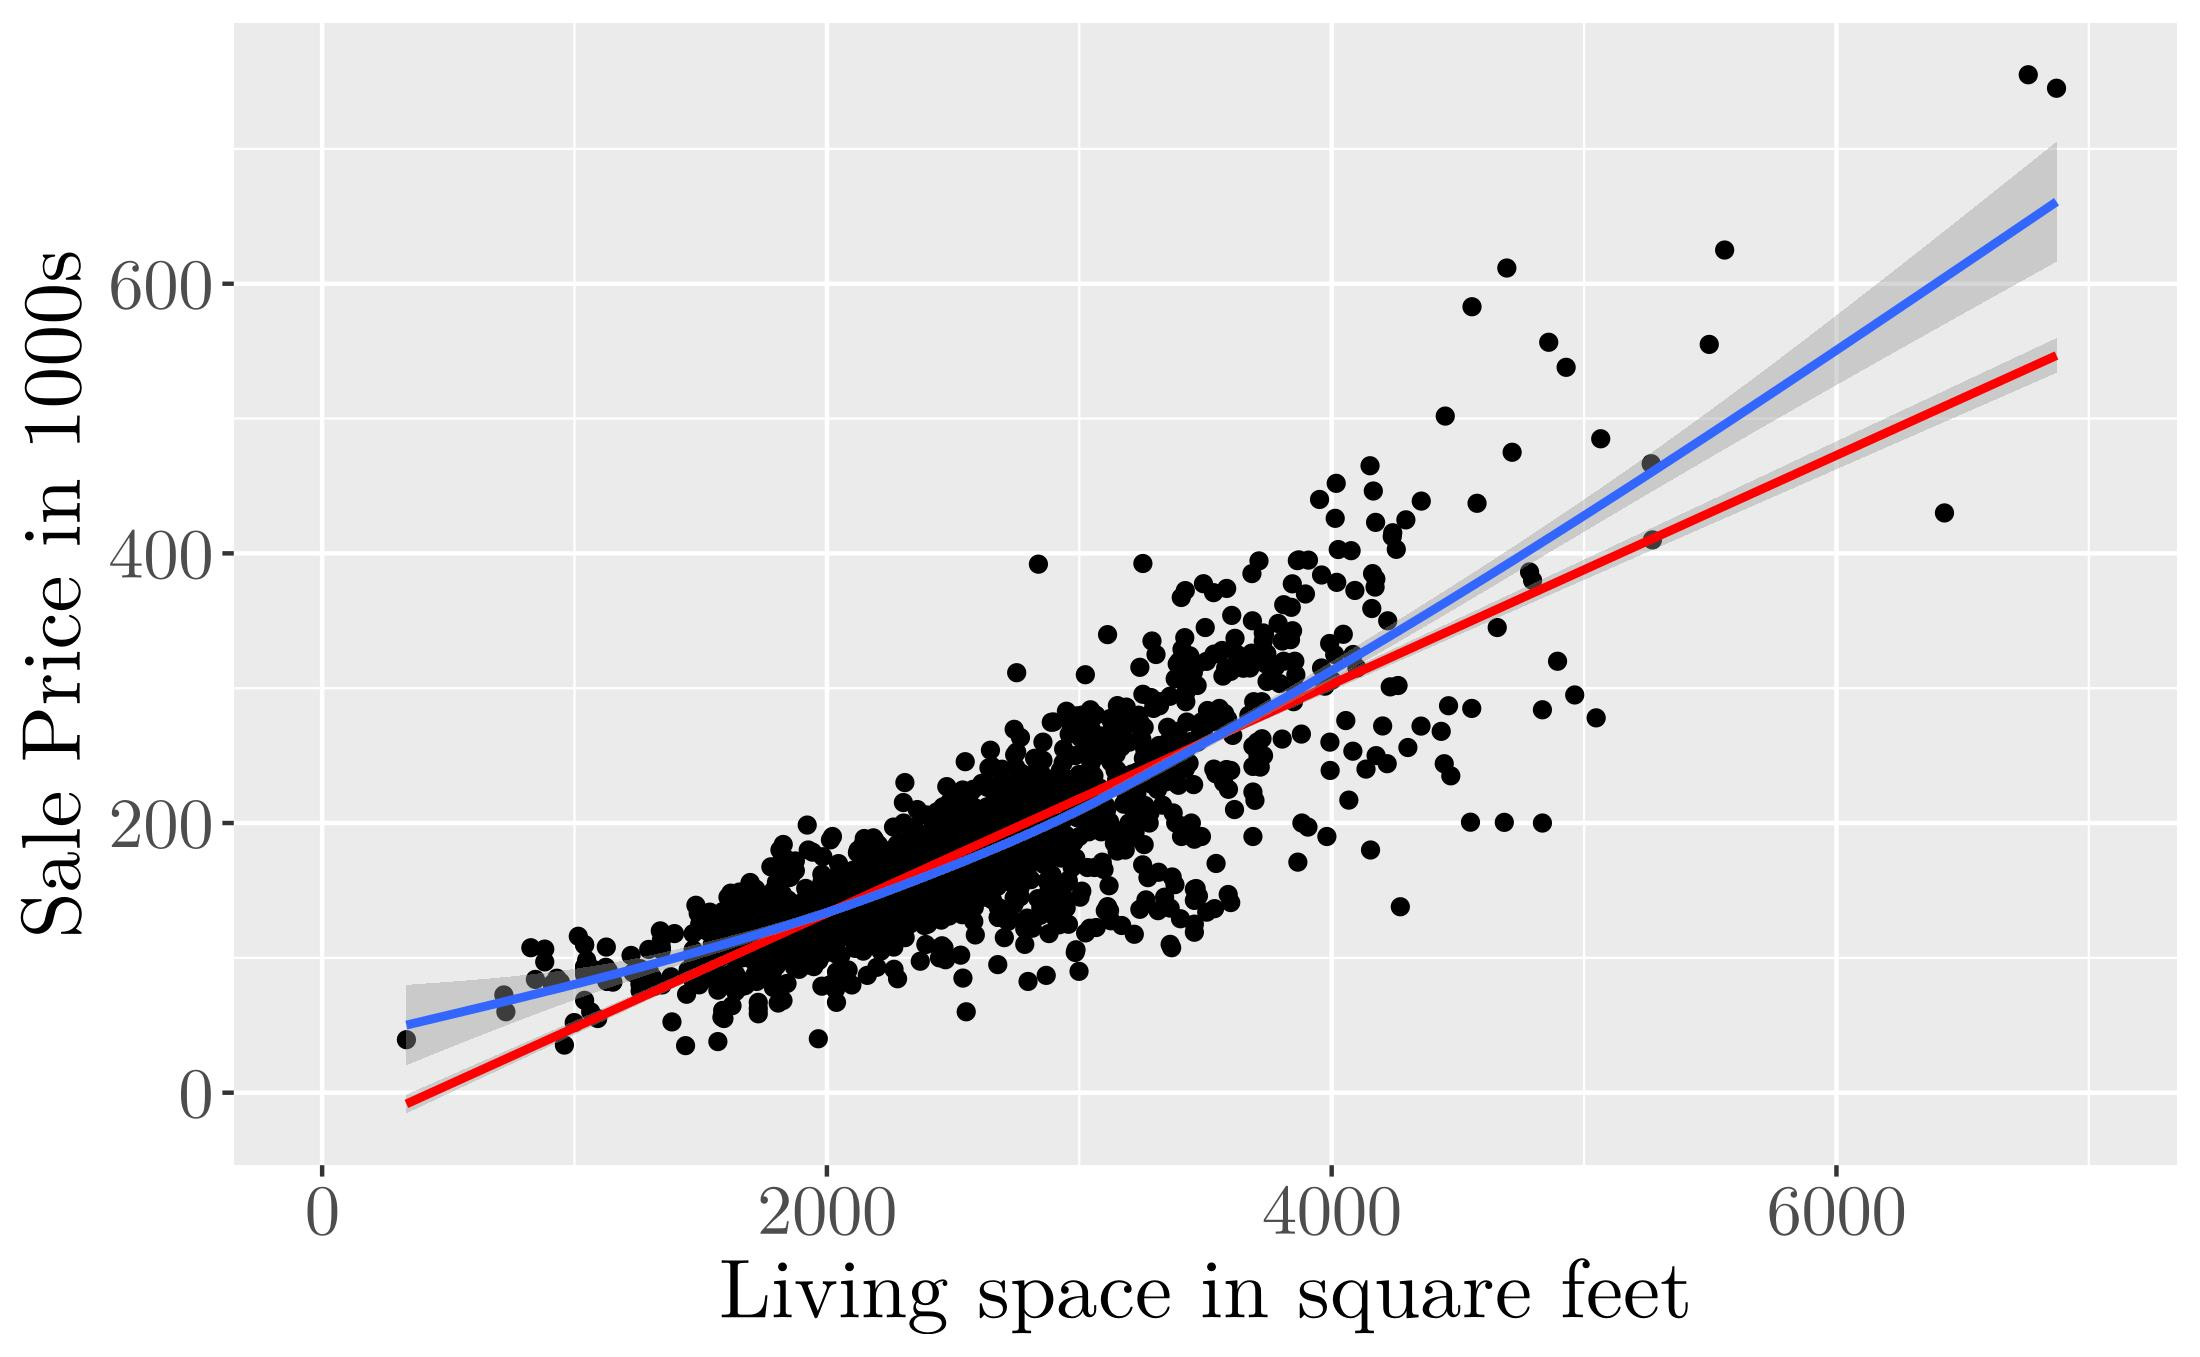
\includegraphics[scale=0.325]{"/home/angelo/Documents/Uni/Courses/Advanced Statistics and programming/Assignments/assignment1/Code/h1.jpg"}
         \small
         \caption{Positive association of total Living Space \& Sale Price \& optimal line; range [0, 7000]}
         \label{fig:y equals x}
     \end{subfigure}
     \hfill
     \begin{subfigure}[b]{0.45\textwidth}
         \centering
         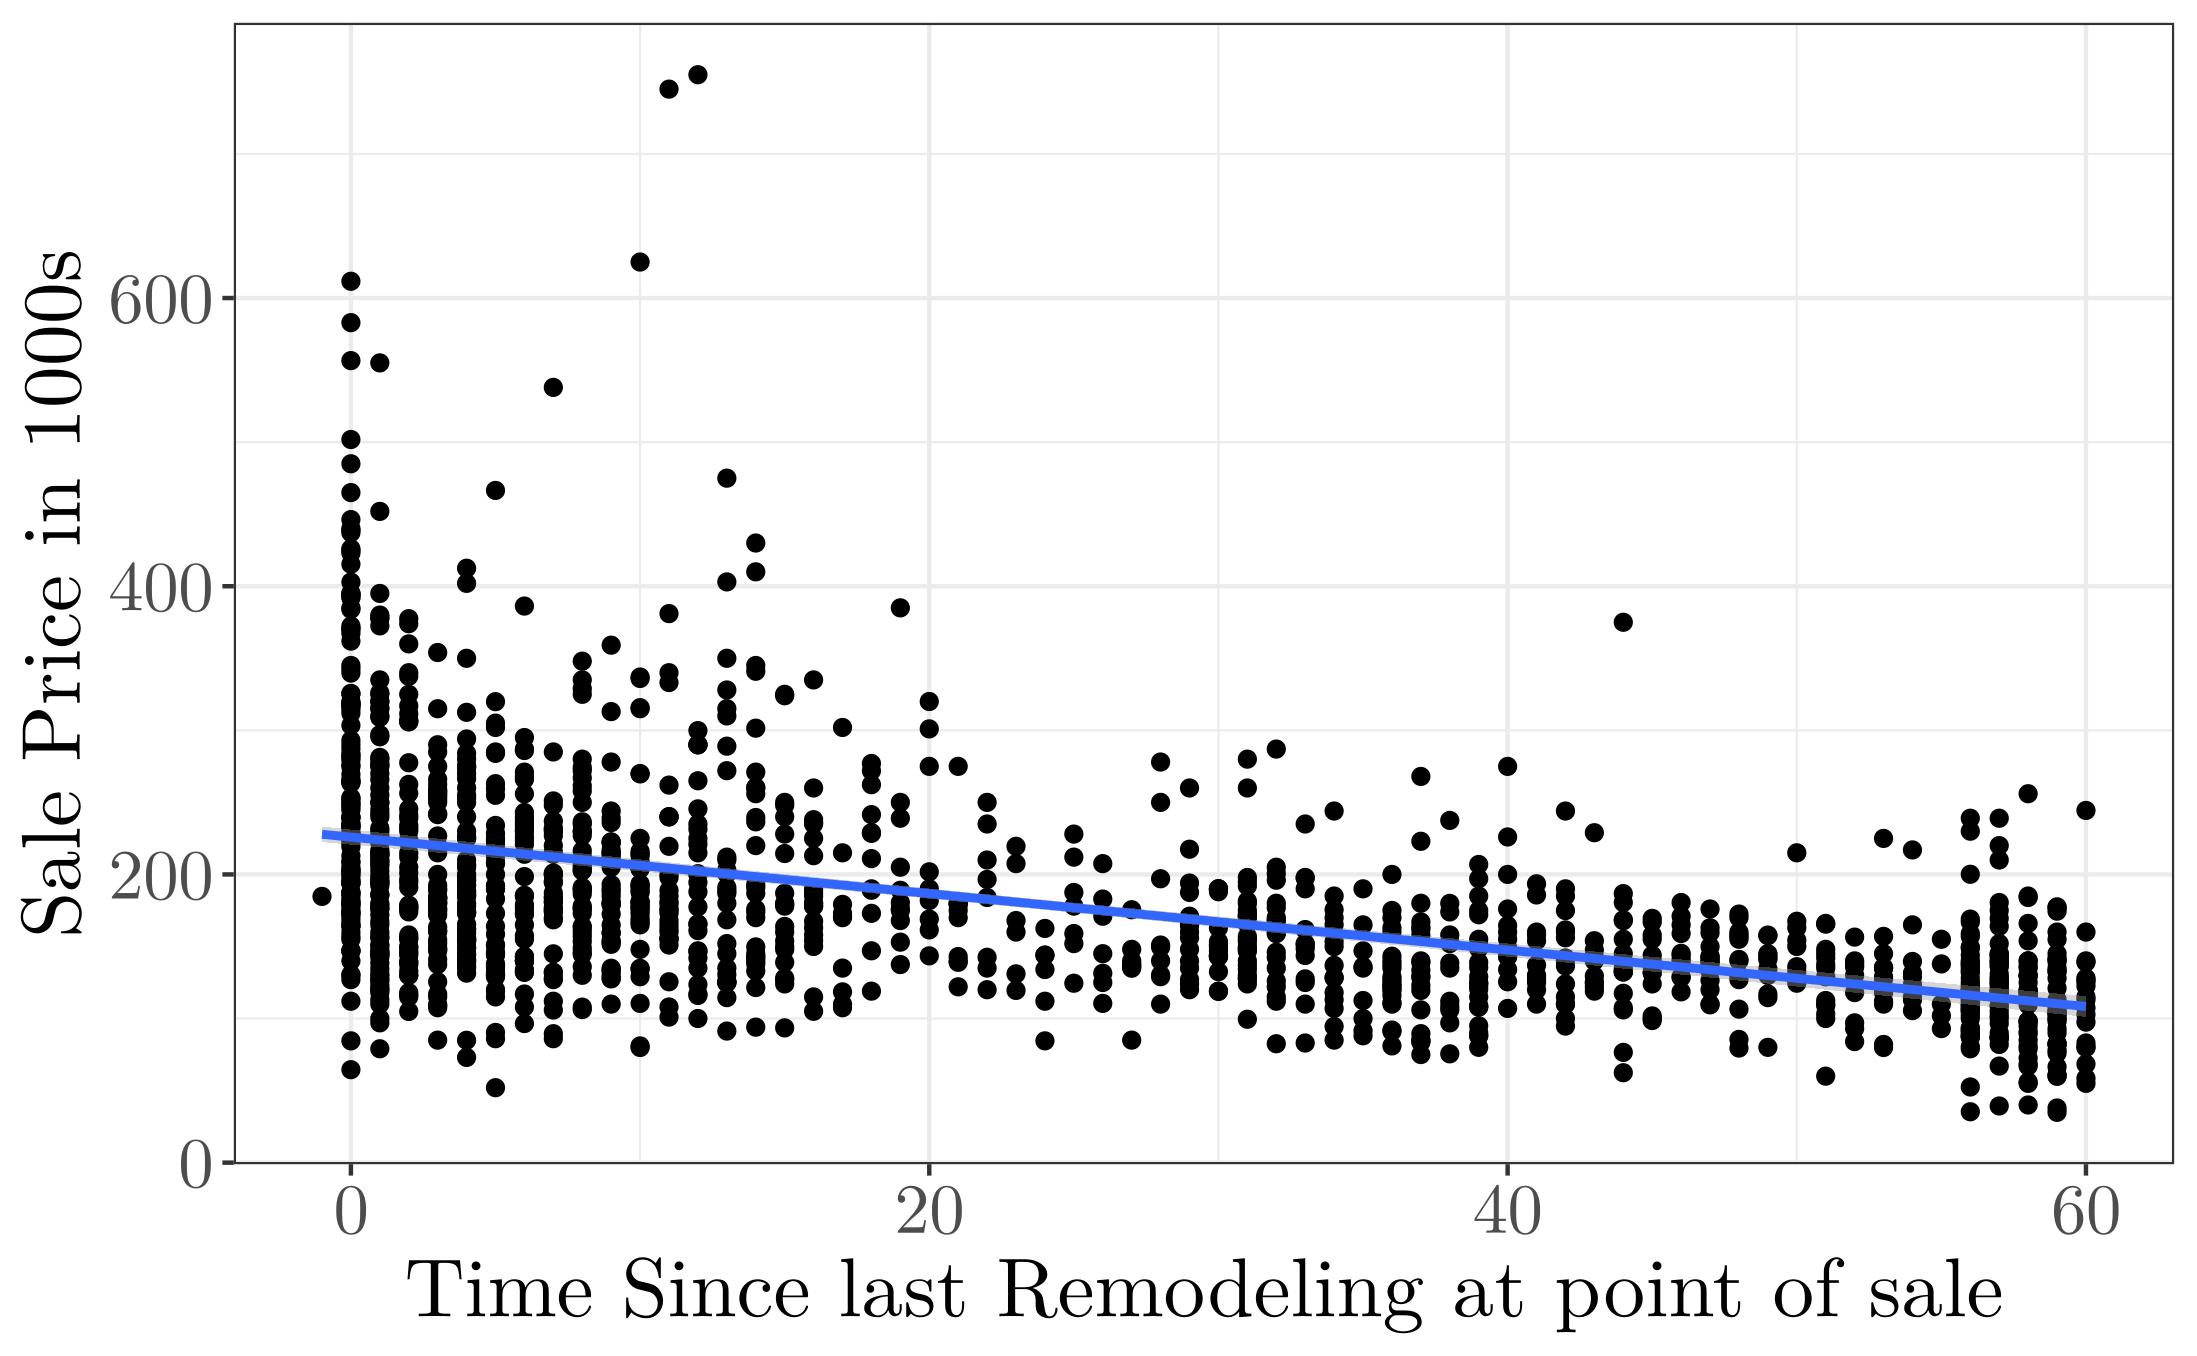
\includegraphics[scale=0.325]{"/home/angelo/Documents/Uni/Courses/Advanced Statistics and programming/Assignments/assignment1/Code/h3.jpg"}
         \small
         \caption{Positive association of total Living Space \& Sale Price }
         \label{fig:three sin x}
     \end{subfigure}
     \hfill
     \begin{subfigure}[b]{0.45\textwidth}
         \centering
         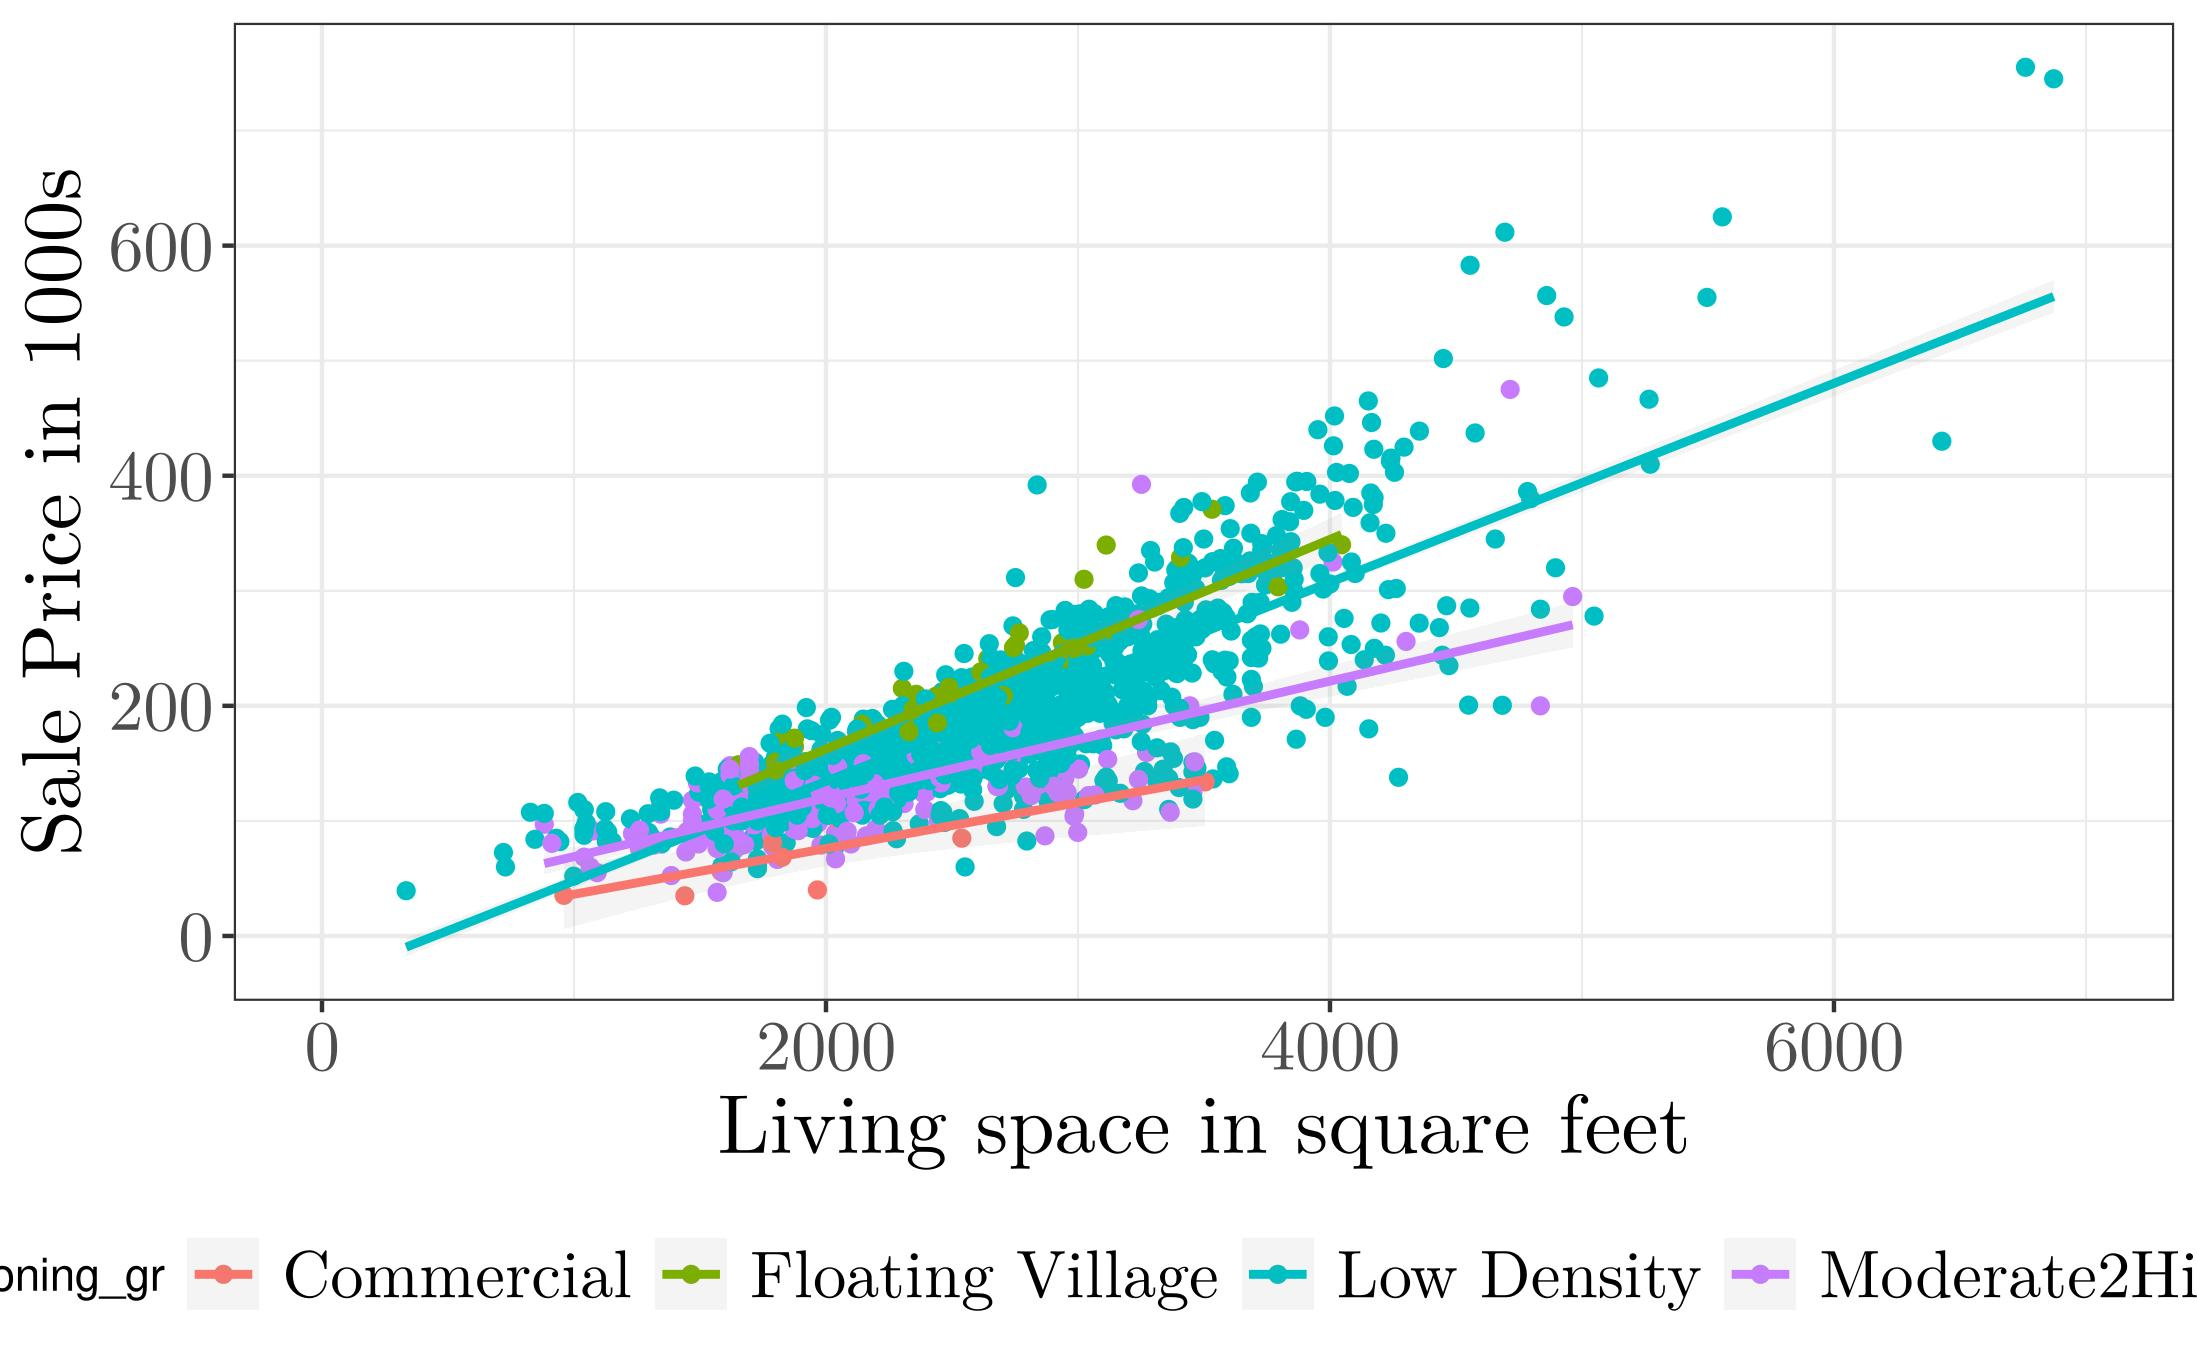
\includegraphics[scale=0.35]{"/home/angelo/Documents/Uni/Courses/Advanced Statistics and programming/Assignments/assignment1/Code/h2.2.jpg"}
         \small
         \caption{Positive association of total Living Space \& Sale Price; range [0, 7000]}
         \label{fig:five over x}
     \end{subfigure}
     	\small
        \caption{Three Hypothesis Graphs displaying their repective association with the outcome variable}
        \label{fig:three graphs}
\end{figure}


Finally, the plots are to be considered in the context of the hypothesis in the next section. 



\section{Theoretical model and OLS assumptions}
\subsection{Hypotheses}
Based on the plots generated during the EDA, a mini theory was created to explain the variation in the sales price of properties (Figure 2). 

\begin{center}
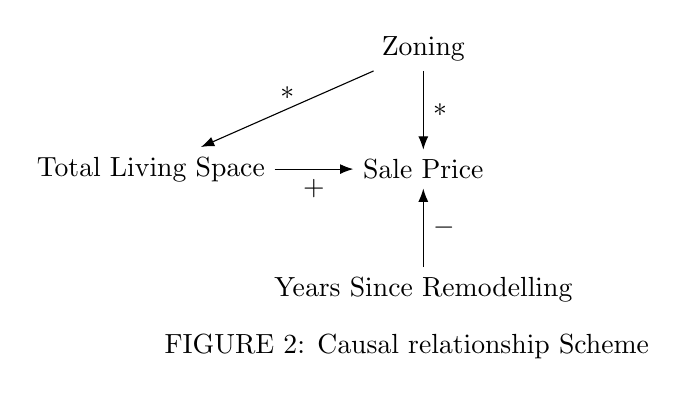
\begin{tikzpicture}
	\centering
 	\node at (3.25,-2.25) {FIGURE 2: Causal relationship Scheme};
    \node (1) at (0,0) {Total Living Space};
	\node (2) [right = of 1] {Sale Price};
	\node (3) [above = of 2] {Zoning};
	\node (4) [below = of 2] {Years Since Remodelling};

	\path (1) edge node[below] {$+$} (2);
	\path (3) edge node[right] {$*$} (2);
	\path (3) edge node[above] {$*$} (1);
	\path (4) edge node[right] {$-$} (2);
	
\end{tikzpicture}
\end{center}



Based on this model, the following three hypothesis were created. 
\subsubsection{Hypotheses 1}


\indent \paragraph{} \textbf{Figure 1A} displays a potential direct positive association between Total Living Space (IV) and Sale Price (DV), including an optimal fit, showing a small. Thus, one expects that larger houses have a higher sale price. Consequently,we assume that:

\begin{hyp}[H\ref{hyp:first}] \label{hyp:first}
Total living space (IV) has a direct postive association with Sales Price (DV)
\end{hyp}

% plot hypothesis 
\begin{center}
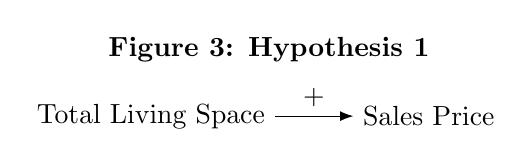
\begin{tikzpicture}
	\centering
 	\node at (1.5,0.85) {\textbf{Figure 3: Hypothesis 1}};
 	\node (1) at (0,0) {Total Living Space};
	\node (2) [right = of 1] {Sales Price};
	\path (1) edge node[above] {$+$}(2);
\end{tikzpicture}
\end{center}


\indent \paragraph{} Subsequently, when taking the Zoning (MSZoning or MSZoning\_grouped - IV) into account to reflect the administrative borderrs of the Ames districts, larger houses in more densly populated areas of the city appear to have a lower price when compared to houses of same size in less densly populated areas as can be seen in \textbf{Plot XXXX2}. This suggests a separation between "downtown less affluent areas" and "suburban affluent areas"\footnote{As an extention\: we will test whether the groups of Neighborhoods generally stay in the same zoning category; if Neighborhoods and Zoning are not related (so eg 50 \% of one neighborhood is in rural zone while the other part is in moderately populated zone) then we have a problem that this woudl induce a bias. Otherwise, we can just proceed.} and concludes in the hypothesis that

\begin{hyp}[H\ref{hyp:second}] \label{hyp:second}
Zoning moderates (MIV) the direct postive association of Total Living Space (IV) and Sale Price (DV). The association of Space and Sale Price is proposed to be weaker for more densly populated areas than for more rural areas. 
\end{hyp}

%fgure h2
\begin{center}


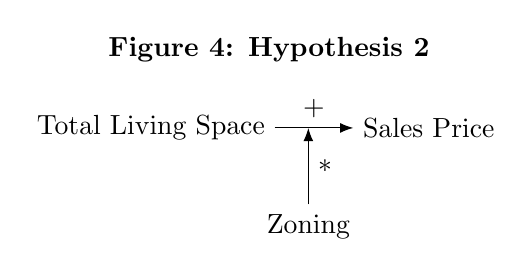
\begin{tikzpicture}
	\centering
 	\node at (1.5,1) {\textbf{Figure 4: Hypothesis 2}};
 	\node (1) at (0,0) {Total Living Space};
	\node (2) [right = of 1] {Sales Price};
	\node (3) at (2,-1.25) {Zoning};
	
	\coordinate (4) at (2,0);
	
	\path (1) edge node[above] {$+$}(2);
	\path (3) edge node[right] {$*$}(4);
\end{tikzpicture}
\end{center}

\indent \paragraph{} As can be observed on Figure 1c, older the houses 8not renovated (IV), are associated with lower sales  prices (DV). Thus, the final hypothesis corresponds to:\footnote{It is notable, that more complex analysis will be considered in part 4 \& 5, such as the moderating effect of Years Since remodeling on the association of Quality and Sale price} 


\begin{hyp}[H\ref{hyp:third}] \label{hyp:third}
Years Since Remodeling (M-IV) or Construction has an amplyfiying effect on the direct postive effect of Quality (IV) and Sale Price (DV)
\end{hyp}

% figure h3
\begin{center}
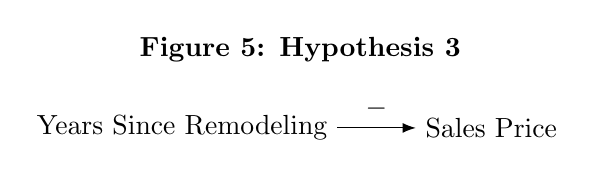
\begin{tikzpicture}
	\centering
 	\node at (1.5,1) {\textbf{Figure 5: Hypothesis 3}};
 	\node (1) at (0,0) {Years Since Remodeling};
	\node (2) [right = of 1] {Sales Price};
	%\node (3) at (1.25,-1.12) {Years Since Remodeling};
	
	%\coordinate (4) at (1.25,0);
	\path (1) edge node[above] {$-$}(2);
	%\path (3) edge node[right] {$-$}(4);
\end{tikzpicture}
\end{center}

%$$ {SalePrice} = \alpha + \beta_{1} TotLivingSpace - \beta_{2}  TotLivingSpace^2 + \beta_{3}  Quality + \beta_{4}  Zoning_{Low Density} + \beta_{5}  Zoning_{Other} + \beta_{6}  YearsSinceRemodeling + \beta_{7}  LotArea + \beta_{8} TotLivingSpace*Zoning_{Low Density} + \beta_{9} TotLivingSpace*Zoning_{Other} +\epsilon$$



\textbf{IMPORTANT: DO YOU INCLUDE A QUADRATIC TERM IN THE POPULATION REGRESSION MODEL???? NO! BUt make more equations explaining each quadartic term and represent the interaction effects etc adn what not }

(2-1)$$ {SalePrice} = \alpha + \beta_{1} TotalLivingSpace - \beta_{2}  Zoning - \beta_{3}  YearsSinceRemodeling +\epsilon$$ (2-1)



\subsection{Assumptions}


\indent A1: The linearity of model parameters and error term assumption suggests that a) the functional form of the underlying population regression model is linear and additive. Thus, this assumption is generally assumed to hold, i.a. not having introduced quadratic or polynominal (by parameter) terms into the population regression equation (2-1). However as Figure 1b shows, there might be a quadratic relationship present between Total Living Area and Sale Price. The reason why this might be the case may be that with increasion values for x ([X = x]), the effect of X on Y increases, which would be represented in later regression models by an additional quadratic term in the regression equation. However, as will be shown in later parts, this can be (partially) remedied.

\indent A2: Full rank assumes that no independent variable can be a linear function of other independent variables; e.g.a 2-dimensional sphere might be compressed to a line, figuratively speaking, meaning that there is no optimal (or none at all) solution for the parameters in question. This first part of the assumtion might easily be violated when not dropping a "comparative" category of a categorical varaible. However, violations of full rank might also come in the form of multicollinearity. Multicollinearity is the "almost" violation of the full rank violation as a given variable may, for isntance, be highly correlated with another given variable. This way the sphere is almost compressed to a single line, which leads to a multitute of problems regarding inference of the model: primairly, the standard errors of the model become unstable to the inclusion of other explanatory or control variables. Multicollinearity is almost always present with observational data (actually making regression interesting in the first place); however, the extend is more relevant. For example might be if we included the Total Linving Space and the TotalNumberofRooms, both of which will be strongly correlated. Further tests will be conducted to probe for this assumption violation. 


\textbf{in what direction is the estimator baised when this variable is left out}

A3: This assumption is referred to as mean independence (or exogeniety); assuming no correlation/systematic association between independent variables and residuals (or conditional mean error is dependent on independent variables). Thus this assumption might induce a bias/ or reduce consistency of the estimator and is, thus, critical to the model itself. A common way, this variable is violated is via unobserved confounders or ommitted variables. If a given variable is left out, part of the error term can be explained by a given variable which suffers under the influence of the confounder. An example in this case will be the missign information regariding crime by the area a property is located. It is obvious that higher crime levels will reduce the value in a given area. Thus, given a certain Neighborhood in question, part of the variance that would have been explained by the Crime variable is now falsely attributed to Neighborhood, biasing the estimate.
Omitted variables bias the estimate of the population coefficient  either up or down, thereby reducing the consistency of the estimate. 

A4: The error term has a constant variance for each observation expected! --> heteroscedasticity

The assumption of homoscedasticity assumes constance variance of each observation. However, if the variance of the estimate is varying we face heteroscedastic variances. While this is not necessarily problematic regarding the estimated parameter (coefficient), heteroscedastictiy impacts the standard errors of the estimate, leading to problems regarding inference; heteroscedastitiy can lead to both type I and II error. In this research, this violation might occur if the eg. sales prices vary stronger for large houses than for small houses. The resulting (averaged) standard error would neither be rebresenative for small and large house standard errors and, thus, inference itself.
\textbf{NOTE AUTOCORRELATION AND YEARS SINCE BUILT}

Generally, as the sample size increases, this assumption becomes less important for the estimate itself, considering that OLS is a consistent estimator; which is the case here (N is quite large). However, heteroscedastictiy may lead to problems regarding inference, as the standard error of the estimate may still be biased. As such, solutions will be later implemented to control for such violations.



A5: Data generation: xi can be random or fixed; the data was collected for predictive purposes so we might not be able to veryfy this. As the data was not generated via a random experiment,none of the variables at hand are \textbf{random variables}
Due to the data originating from sales in a town in Iowa (Ames), we have to assume that the data at ahnd is "fixed". Thus, inference regardign a wider population cannot be made from this data, as its fixed nature only applies to small towns in the mid-western USA. However, we can assume that the fixed variables collected are measured without error; particualrly as the sample collected can be somewhat representative of the wider popualtion of small towns in the mid-western USA. 


generally, due to the nature of the data, being a 

\textbf{in order to }

A6: This assumption regards inference; if the residuals do not follow a standard normal distribution, this might result in incorrect decisions as the distribution might for instance be "fatter" in the tails, resulting in potentially Type I or Type II errors. This might be the case if for instance we do not have a lot of observations for e.g. subcategories. Subsequently, the resulting inference might be biased. However, as the sample size increases, most distributions approach the normal form. 
However, in order to answer the question, this assumtion is violated via i.a. large amounts of outliers. As can be seen in Figure 1a the range goes from 0 to 7000 square feet, thus, ommits two extreme outliers.


\section{OLS regression and model fit}
\subsection{Normal Regression}

\begin{table}[!htbp] \centering 
\begin{adjustwidth}{0.5cm}{-0cm}
\begin{threeparttable}
\small
\captionsetup{font=small, justification=raggedright,singlelinecheck=false}
\caption{\textsc{Merged Standardized Regresson Results containing both standardized and unstandardized coefficients FINAL VERSION 3 models complete yay}}
\centering 
  \label{}
\small 
\begin{tabular}{@{\extracolsep{-7pt}}lcccccc} 
\\[-5.8ex]\hline 
\hline \\[-1.8ex] 
 & \multicolumn{6}{c}{\textit{Dependent variable:}} \\ 
\cline{2-7} 
\\[-1.8ex] & \multicolumn{2}{c}{SalePrice} & \multicolumn{2}{c}{SalePrice} & \multicolumn{2}{c}{ln\_SalePrice} \\ 
\\[-1.8ex] & Model (1) & Std. Coef.& Model (2) & Std. Coef.&  Model (3) & Std. Coef.\\ 
\hline \\[-1.8ex] 
 Constant & 15.229 &  & 24.550 &  & 3.584$^{***}$ &  \\ 
  & (25.697) &  & (24.541) &  & (0.114) & \\ 
  & & & & & & \\ 
 Living Space & 0.035$^{***}$ & 0.362$^{***}$ & 0.038$^{***}$ & 0.393$^{***}$ & 0.0003$^{***}$ & 0.684$^{***}$ \\ 
  & (0.002) & & (0.005) & & (0.00002) &  \\ 
  & & & & & & \\ 
 Years Since Remodeling & $-$0.492$^{***}$ & $-$0.128$^{***}$ & $-$0.493$^{***}$ & $-$0.128$^{***}$ & $-$0.003$^{***}$ & $-$0.170$^{***}$ \\ 
  & (0.056) &  & (0.051) &  & (0.0002) &  \\ 
  & & & & & & \\ 
 Low Dens. Zone & 16.640$^{***}$ & 0.086$^{***}$ & $-$31.118$^{***}$ & $-$0.160$^{***}$ & 0.077$^{**}$ & 0.079$^{**}$ \\ 
  & (2.753) &  & (8.368) & & (0.039) &  \\ 
  & & & & & & \\ 
 Commercial Zone & $-$25.251$^{**}$ & $-$0.026$^{**}$ & $-$35.782 & $-$0.037 & $-$0.673$^{***}$ & $-$0.139$^{***}$ \\ 
  & (11.881) &  & (35.624) &  & (0.165) &  \\ 
  & & & & & & \\ 
 Floating Zone & 18.710$^{***}$ & 0.049$^{***}$ & $-$8.247 & $-$0.021 & 0.127 & 0.065 \\ 
  & (5.258) & & (22.841) & & (0.106) &  \\ 
  & & & & & & \\ 
 Lot Area & 0.001$^{***}$ & 0.074$^{***}$ & 0.005$^{***}$ & 0.616$^{***}$ & 0.00002$^{***}$ & 0.404$^{***}$ \\ 
  & (0.0001) &  & (0.0005) &  & (0.00000) &  \\ 
  & & & & & & \\ 
  
 I(Living Space$\hat{\mkern6mu}$2) &  &  & $-$0.00000 & $-$0.002 & $-$0.00000$^{***}$ & $-$0.234$^{***}$ \\ 
  &  &  & (0.00000) &  & (0.000) &  \\ 
  & & & & & & \\ 
 Living Space:Low Dens. Zone &  &  & 0.019$^{***}$ & 0.308$^{***}$ & 0.00002 & 0.058 \\ 
  &  &  & (0.004) & & (0.00002) &  \\ 
  & & & & & & \\ 
 Living Space:Commercial Zone &  &  & 0.0001 & 0.0002 & 0.0002$^{**}$ & 0.067$^{**}$ \\ 
  &  &  & (0.017) & & (0.0001) & \\ 
  & & & & & & \\ 
 Living Space:Floating Zone &  &  & 0.013 & 0.088 & 0.00002 & 0.022 \\ 
  &  &  & (0.009) &  & (0.00004) & \\ 
  & & & & & & \\ 
 Living Space:Lot Area &  &  & $-$0.00000$^{***}$ & $-$0.647$^{***}$ & $-$0.000$^{***}$ & $-$0.396$^{***}$ \\ 
  &  &  & (0.00000) &  & (0.000) &  \\ 
  & & & & & & \\ 
  Year Sold & YES & YES & YES & YES & YES & YES \\ 
  %&  & &  &  \\ 
  % & & & & \\ 
  Overall Quality Rating & YES & YES & YES & YES & YES & YES \\  
  % & (32.730) & (32.730) & (30.513) & (30.513) \\ 
  %& & & & \\ 
  Building Type & YES & YES & YES & YES & YES & YES \\ 
  %& (2.654) & (2.654) & (2.501) & (2.501) \\ 
  % & & & & \\ 
\hline \\[-1.8ex]  
\end{tabular} 
%%%%%%%
\small 
\centering
\begin{tabular}{@{\extracolsep{19pt}}lcccccc} 
R$^{2}$ && 0.803 &   0.836 &  0.861   \\ 
Adjusted R$^{2}$ && 0.800 &  0.833 &   0.858  \\ 
Residual Std. Error && 35.548  & 32.488  & 0.150   \\ 
df Residual Std. Error && (df = 1439)  & (df = 1434) & (df = 1434)\\
F Statistic& & 292.393$^{***}$    & 291.609$^{***}$   & 354.941$^{***}$    \\ 
df F Statistic && (df = 20; 1439)  & (df = 25; 1434)  & (df = 25; 1434)   \\
\hline 
\hline \\[-3.5ex] 
\end{tabular} 
\begin{tablenotes}[para,flushleft]
      \small
      \item\textit{Note:} N = 1460. All observations included in any model. OLS estimates, robust standard errors in parentheses.*** p$<$0.01, ** p$<$0.05, * p$<$0.1. This table reportes the (unstandardized) regression results for the Model (1) excluding any interaction effects \& and inclduing those interaction effects in Model (3). The corresponding standardized coefficients can be foudn in Std.Model (2) \& (3). For complementary regression models \textbf{see appendix}. The comparison category in "Zone" (IV) is "Moderate-to-High Density". Years in date range is 2006 to 2010. 
    \end{tablenotes}
\end{threeparttable}
\end{adjustwidth}
%
\end{table}


\textbf{NOTE: This regression table shifts from including interaction effects, scaling, etc from one model to the other; I chose to 
The choice to not include incremental models was done to keep the analysisi concise. In the appendix one can see that the $Adj-  R²$ increases also only due to the inclusion of further control variables without interaction terms. Nonetheless, also the interaction terms imrpove on the model fit (with and without control variables). Finally, Model (3) \& (4) include all interaction effects and scaled variables (such as LN SalePrice) as no model shows a lower isses in this regard.} Thus, only the simple multi-variate model and an extensive model was displayed.









Table 2 reports a simplified (1) and complex model (3), containing all corresponding interaction effects and control varaibles \footnote{It is notable, that more complex analysis will be considered in part 4 \& 5, such as the moderating effect of Years Since remodeling on the association of Quality and Sale price}


Table 2 reportes the (unstandardized) regression results for the Model (1) excluding any interaction effects \& and inclduing those interaction effects in Model (3).\footnote{It is notable, that more complex analysis will be considered in part 4 \& 5, such as the moderating effect of Years Since remodeling on the association of Quality and Sale price} The corresponding standardized coefficients can be foudn in Std.Model (2) \& (3).\footnote{It may be noted that the Sale Price will be log scaled in Part 4; the interaction term of Total Living Space with itself was already included in this section as I assume that part 3 is mainly about the independent variables demonstrating once the noremal interpretation; as such a complete model will be provided in part 4, containing the log scaled version of the independent}





he study of Sales Price of property in Ames, Iowa, has shown that the Total Living Area has a significant postive effect on the Sales Pri


Table 3 reports the regression results of  for the four sucessively extensive models starting from only the independent variable from Figure 2, then adding interaction terms in model (2), control variables in model (3) without interactions, and a complete model (4) including interaction terms, which will be discussed below. All four models have been reported to demonstrate that for the main indepenent variables (see Figure 2) the coefficients and Standard Errors are stable to the inclusion of control variables and interaction terms.\footnote{Please note that log scaling of the dependent variable was not done on purpose at this point due to this task falling into part 4 of this assignment}
Considering model (4) as the Complete model
Specifically, this research shows that the association Total Living Space and Sale Price is positive and  statistically significant (($\hat{\beta}$ = 0.040, $p$ = 0.01)


he study of Sales Price of property in Ames, Iowa, has shown that the Total Living Area has a significant postive effect on the Sales Pri

Overall, the inclusion of the interaction of Zone (M-IV) and Total Living Area (IV), in addition to introducing a quadratic term of Total Living Area (IV) improves the model fit sighlty from 


\subsection{Standardized Regression Coefficients and Effect Size}










\section{Diagnostic checking}
\textbf{It is notable, that more complex analysis will be considered in part 4 \& 5, such as the moderating effect of Years Since remodeling on the association of Quality and Sale price}

\textbf{IMPORTANT: FOR PART 4 CREATE A TABLE THAT CONATINS OLS ROBUST TO STANDARD ERRORS!!!! (THIS EXACT TABLE!!)}

\textbf{IMPOIRTANT HERE WE WILL NOT ONLY COMPARE THE BASE MODEL WITHOUT SCALE SALE PRICE, But also THE FULL MODEL WITH SCALED EVERYTHING and corrections for standard errors }

to do: 1) log scale outcome variable because it is a an important factor; 2) secondly, the quadractic term of Total livign space is already in the part before, but here the rational is different was we were only talking about the independent variables in that case. as such I did not consider the total living area to be an issue here 




\section{Subset analyses}
\textbf{In this analysis we will examine further interaction and subsection analysis; such as quality as a numeric variable}














 
 

\textbf{MERGE THE STANDARDZIDER AND UNSTANDARDIZED TABLE}




\begin{table}[!htbp] \centering 
\begin{adjustwidth}{-0.0cm}{-0cm}
\begin{threeparttable}
\small
\captionsetup{font=small, justification=raggedright,singlelinecheck=false}
\caption{\textsc{Merged Standardized Regresson Results containing both standardized and unstandardized coefficients FINAL VERSION BACKUP}}
\centering 
  \label{}
\small 
\begin{tabular}{@{\extracolsep{-1pt}}lcccc} 
\\[-5.8ex]\hline 
\hline \\[-1.8ex] 
 & \multicolumn{4}{c}{\textit{Dependent variable:}} \\ 
\cline{2-5} 
\\[-1.8ex] & \multicolumn{2}{c}{Sale Price} & \multicolumn{2}{c}{ln(Sale Price)} \\ 
\\[-1.8ex] & Model (1) & Std.Model (2) & Model (3) & Std.Model (4)\\ 
\hline \\[-1.8ex] 
 Constant & 15.229 & / & 3.584$^{***}$ & / \\ 
  & (25.697) &  & (0.114) &  \\ 
  & & & & \\ 
 Total Living Space & 0.035$^{***}$ & 0.362$^{***}$ & 0.0003$^{***}$ & 0.684$^{***}$ \\ 
  & (0.002) &  & (0.00002) &  \\ 
  & & & & \\ 
 Years Since Remodelling & $-$0.492$^{***}$ & $-$0.128$^{***}$ & $-$0.003$^{***}$ & $-$0.170$^{***}$ \\ 
  & (0.056) &  & (0.0002) &  \\ 
  & & & & \\ 
 Low Density Zone & 16.640$^{***}$ & 0.086$^{***}$ & 0.077$^{**}$ & 0.079$^{**}$ \\ 
  & (2.753) &  & (0.039) &  \\ 
  & & & & \\ 
 Commercial Zone & $-$25.251$^{**}$ & $-$0.026$^{**}$ & $-$0.673$^{***}$ & $-$0.139$^{***}$ \\ 
  & (11.881) &  & (0.165) &  \\ 
  & & & & \\ 
 Floating Zone & 18.710$^{***}$ & 0.049$^{***}$ & 0.127 & 0.065 \\ 
  & (5.258) &  & (0.106) &  \\ 
  & & & & \\ 
 I(Total Living Area$\hat{\mkern6mu}$2) &  &  & $-$0.00000$^{***}$ & $-$0.234$^{***}$ \\ 
  &  &  & (0.000) &  \\ 
  & & & & \\ 
 Lot Area & 0.001$^{***}$ & 0.074$^{***}$ & 0.00002$^{***}$ & 0.404$^{***}$ \\ 
  & (0.0001) &  & (0.00000) &  \\ 
  & & & & \\ 
 "Total Living Area":"Low Density Zone" &  &  & 0.00002 & 0.058 \\ 
  &  &  & (0.00002) &  \\ 
  & & & & \\ 
 "Total Living Area":"Commercial Zone" &  &  & 0.0002$^{**}$ & 0.067$^{**}$ \\ 
  &  &  & (0.0001) &  \\ 
  & & & & \\ 
 "Total Living Area":"Floating Zone" &  &  & 0.00002 & 0.022 \\ 
  &  &  & (0.00004) &  \\ 
  & & & & \\ 
 "Total Living Area":"Lot Area" &  &  & $-$0.000$^{***}$ & $-$0.396$^{***}$ \\ 
  &  &  & (0.000) &  \\ 
  & & & & \\ 
  Year Sold & YES & YES & YES & YES \\ 
  %&  & &  &  \\ 
  % & & & & \\ 
  Overall Quality Rating & YES & YES & YES & YES \\  
  % & (32.730) & (32.730) & (30.513) & (30.513) \\ 
  %& & & & \\ 
  Building Type & YES & YES & YES & YES \\ 
  %& (2.654) & (2.654) & (2.501) & (2.501) \\ 
  % & & & & \\ 
\hline \\[-1.8ex] 
R$^{2}$ & 0.803 & 0.803 & 0.861 & 0.861 \\ 
Adjusted R$^{2}$ & 0.800 & 0.800 & 0.858 & 0.858 \\ 
Residual Std. Error & 35.548 & 35.548  & 0.150  & 0.150 \\
df Residual Std. Error & (df = 1439) & (df = 1439) & (df = 1434) & (df = 1434)\\
F Statistic & 292.393$^{***}$  & 292.393$^{***}$  & 354.941$^{***}$  & 354.941$^{***}$  \\ 
df F Statistic & (df = 20; 1439) & (df = 20; 1439) & (df = 25; 1434) & (df = 25; 1434) \\
\hline 
\hline \\[-3.5ex] 
\end{tabular} 
\begin{tablenotes}[para,flushleft]
      \small
      \item\textit{Note:} N = 1460. All observations included in any model. OLS estimates, robust standard errors in parentheses.*** p$<$0.01, ** p$<$0.05, * p$<$0.1. This table reportes the (unstandardized) regression results for the Model (1) excluding any interaction effects \& and inclduing those interaction effects in Model (3). The corresponding standardized coefficients can be foudn in Std.Model (2) \& (3). For complementary regression models \textbf{see appendix}. The comparison category in "Zone" (IV) is "Moderate-to-High Density". Years in date range is 2006 to 2010. 
    \end{tablenotes}
\end{threeparttable}
\end{adjustwidth}
%
\end{table}






\end{document}
